%%% Hlavní soubor. Zde se definují základní parametry a odkazuje se na ostatní části. %%%

%% Verze pro jednostranný tisk:
% Okraje: levý 40mm, pravý 25mm, horní a dolní 25mm
% (ale pozor, LaTeX si sám přidává 1in)
\documentclass[12pt,a4paper]{report}
\setlength\textwidth{145mm}
\setlength\textheight{247mm}
\setlength\oddsidemargin{15mm}
\setlength\evensidemargin{15mm}
\setlength\topmargin{0mm}
\setlength\headsep{0mm}
\setlength\headheight{0mm}
% \openright zařídí, aby následující text začínal na pravé straně knihy
\let\openright=\clearpage

%% Pokud tiskneme oboustranně:
% \documentclass[12pt,a4paper,twoside,openright]{report}
% \setlength\textwidth{145mm}
% \setlength\textheight{247mm}
% \setlength\oddsidemargin{15mm}
% \setlength\evensidemargin{0mm}
% \setlength\topmargin{0mm}
% \setlength\headsep{0mm}
% \setlength\headheight{0mm}
% \let\openright=\cleardoublepage

%% Použité kódování znaků: obvykle latin2, cp1250 nebo utf8:
\usepackage[utf8]{inputenc}

%% Ostatní balíčky
\usepackage{graphicx}
\usepackage{amsthm}
\usepackage{amsfonts}
\usepackage{amsmath}
\usepackage{siunitx}
\usepackage{dirtytalk}


%% Vlastne prikazy
\newcommand{\mb}[1]{\mathbf{#1}}
\newcommand{\mbb}[1]{\mathbb{#1}}

%% Balíček hyperref, kterým jdou vyrábět klikací odkazy v PDF,
%% ale hlavně ho používáme k uložení metadat do PDF (včetně obsahu).
%% POZOR, nezapomeňte vyplnit jméno práce a autora.
\usepackage[unicode]{hyperref}   % Musí být za všemi ostatními balíčky
\hypersetup{pdftitle=Numerical simulation of ferrofluids}
\hypersetup{pdfauthor=Michal Habera}

%%% Drobné úpravy stylu

% Tato makra přesvědčují mírně ošklivým trikem LaTeX, aby hlavičky kapitol
% sázel příčetněji a nevynechával nad nimi spoustu místa. Směle ignorujte.
\makeatletter
\def\@makechapterhead#1{
  {\parindent \z@ \raggedright \normalfont
   \Huge\bfseries \thechapter. #1
/   \par\nobreak
   \vskip 20\p@
}}
\def\@makeschapterhead#1{
  {\parindent \z@ \raggedright \normalfont
   \Huge\bfseries #1
   \par\nobreak
   \vskip 20\p@
}}
\makeatother

% Toto makro definuje kapitolu, která není očíslovaná, ale je uvedena v obsahu.
\def\chapwithtoc#1{
\chapter*{#1}
\addcontentsline{toc}{chapter}{#1}
}

\begin{document}

% Trochu volnější nastavení dělení slov, než je default.
\lefthyphenmin=2
\righthyphenmin=2

%%% Titulní strana práce

\pagestyle{empty}
\begin{center}

\large

Charles University in Prague

\medskip

Faculty of Mathematics and Physics

\vfill

{\bf\Large BACHELOR THESIS}

\vfill

\centerline{\mbox{
\includegraphics[width=60mm]{./img/logo}}}

\vfill
\vspace{5mm}

{\LARGE Michal Habera}

\vspace{15mm}

% Název práce přesně podle zadání
{\LARGE\bfseries Numerical simulation of ferrofluids}

\vfill

% Název katedry nebo ústavu, kde byla práce oficiálně zadána
% (dle Organizační struktury MFF UK)
Mathematical Institute of Charles University

\vfill

\begin{tabular}{rl}

Supervisor of the bachelor thesis: & RNDr. Ing. Jaroslav Hron, Ph.D. \\
\noalign{\vspace{2mm}}
Study programme: & Physics \\
\noalign{\vspace{2mm}}
Specialization: & General Physics \\
\end{tabular}

\vfill

% Zde doplňte rok
Prague 2015

\end{center}

\newpage

%%% Následuje vevázaný list -- kopie podepsaného "Zadání bakalářské práce".
%%% Toto zadání NENÍ součástí elektronické verze práce, nescanovat.


%%% Strana s čestným prohlášením k bakalářské práci

\vglue 0pt plus 1fill

\noindent
I declare that I carried out this bachelor thesis independently, and only with the cited
sources, literature and other professional sources.

\medskip\noindent
I understand that my work relates to the rights and obligations under the Act No.
121/2000 Coll., the Copyright Act, as amended, in particular the fact that the Charles
University in Prague has the right to conclude a license agreement on the use of this
work as a school work pursuant to Section 60 paragraph 1 of the Copyright Act.

\vspace{10mm}

\hbox{\hbox to 0.5\hsize{%
In ........ date ............
\hss}\hbox to 0.5\hsize{%
signature of the author
\hss}}

\vspace{20mm}
\newpage

%%% Na tomto místě mohou být napsána případná poděkování (vedoucímu práce,
%%% konzultantovi, tomu, kdo zapůjčil software, literaturu apod.)


\openright

\noindent
Dedication.

\newpage


%%% Povinná informační strana bakalářské práce

\vbox to 0.5\vsize{
\setlength\parindent{0mm}
\setlength\parskip{5mm}

Název práce:
Numerické simulace ferrotekutin
% přesně dle zadání

Autor:
Michal Habera

Katedra:  % Případně Ústav:
Matematický ústav UK
% dle Organizační struktury MFF UK

Vedoucí bakalářské práce:
RNDr. Ing. Jaroslav Hron Ph.D., Matematický ústav UK
% dle Organizační struktury MFF UK, případně plný název pracoviště mimo MFF UK

Abstrakt:
% abstrakt v rozsahu 80-200 slov; nejedná se však o opis zadání bakalářské práce

Klíčová slova:
% 3 až 5 klíčových slov

\vss}\nobreak\vbox to 0.49\vsize{
\setlength\parindent{0mm}
\setlength\parskip{5mm}

Title:
Numerical simulation of ferrofluids
% přesný překlad názvu práce v angličtině

Author:
Michal Habera

Department:
Mathematical Institute of Charles University
% dle Organizační struktury MFF UK v angličtině

Supervisor:
RNDr. Ing. Jaroslav Hron, Ph.D., Mathematical Institute of Charles University
% dle Organizační struktury MFF UK, případně plný název pracoviště
% mimo MFF UK v angličtině

Abstract:
% abstrakt v rozsahu 80-200 slov v angličtině; nejedná se však o překlad
% zadání bakalářské práce

Keywords:
% 3 až 5 klíčových slov v angličtině

\vss}

\newpage

%%% Strana s automaticky generovaným obsahem bakalářské práce. U matematických
%%% prací je přípustné, aby seznam tabulek a zkratek, existují-li, byl umístěn
%%% na začátku práce, místo na jejím konci.

\openright
\pagestyle{plain}
\setcounter{page}{1}
\tableofcontents

%%% Jednotlivé kapitoly práce jsou pro přehlednost uloženy v samostatných souborech
\chapter*{Introduction}
\addcontentsline{toc}{chapter}{Introduction}

\par Free surface fluid flows and processes involved in a fluid behavior fascinated scientists since the very beginning of the scientific history. Problems as a breakup of a liquid jet, droplet formation and merging, rising bubbles etc. still lacks deeper understanding because of a complex and nonlinear equations governing such phenomena. In addition, they play a role in many industrial processes: \textit{fuel injection, fibre spinning, ink-jet printing etc.} EGGERS

\par The equations for the motion of a fluid formulated in the 19th century came to relevance as computers started to provide number of numerical methods for finding their approximate solutions. However, majority of the methods are well suited for problems involving one-phase flows or fluid-wall interactions, multi-phase flows, fluid-fluid interactions, surface forces and similar issues still remain debated and incomplete.

\par Imagine some usual situation, where a water droplet hanging on a tap is being pulled down by the gravity. From a physical point of view, the behavior and evolution is well described. \textit{Navier-Stokes} equations govern the fluid motion in each phase, water and air separately, while discrete surface forces(surface tension) are balanced with the gravitational, volume force. Mathematically, not only an existence and uniqueness of a solution of the equations was proven, but multiple domains coupled with complex boundary conditions must be taken into account.


\begin{figure}[ht]
\centering
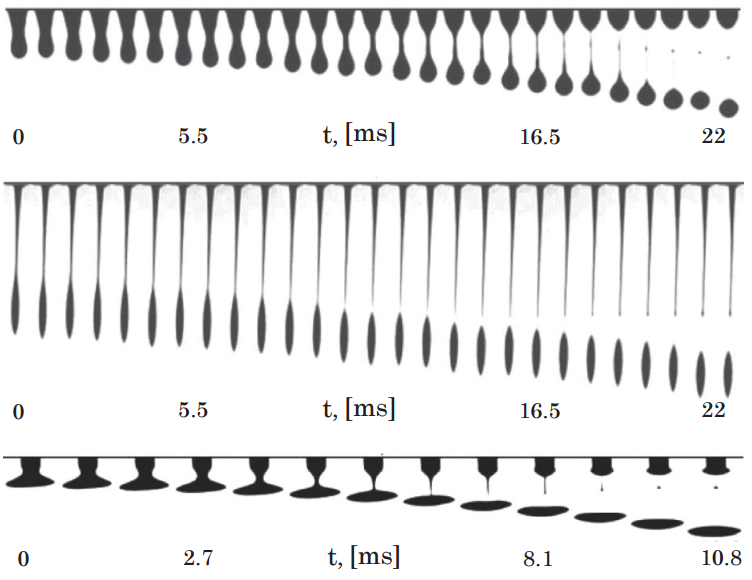
\includegraphics[width=80mm]{img/ferrofluid_motivation.png}
\caption{High-speed image sequence of ferrofluid droplet dripping out of a container. Influence of a magnetic field parallel(middle) and perpendicular(bottom) to the direction of the flow is clearly visible. Taken from [HABERA]}
\end{figure}

\par All these phenomena become even more attractive in terms of \textit{ferrohydrodynamics}. Ferrofluid reacts to magnetic field and changes its shape due to an additional surface force. This entirely changes dynamics of the droplet formation process and it will be the object for our studies.

\par In the first part of the thesis a brief summary of the physical and mathematical model and numerical methods are given. Navier-Stokes equations are solved using the \textit{projection methods} and spatially approximated in sense of weak derivates and \textit{finite element method}. Interface is represented with the \textit{level-set} function, while the conservation of its volume is assured with the reinitialization step.  

\par In the second part we discuss the results of the implemented methods and give a direct comparison of our results with experimental data obtained in HABERA.

\chapter{Ferrofluids}

\section{Introduction}
\section{Ferrohydrodynamics}

\chapter{The Finite element method}

\par In the following sections we give a very brief introduction into the finite element method. 
We also refer more advanced reader who seeks more detail to [3 in LINDBO].

\section{Problem definition}

\par We are interested in a solution of a partial differential equations of the type 
$$\mathcal{L}(u(\mb x)) = f(\mb x),~\forall \mathbf{x}\in\Omega$$
on a given domain $\Omega$, where $\mathcal{L}$ is a linear differential operator, 
$u = u(x_1,\ldots,x_n)=: u(\mb x)$
and
$f = f(x_1,\ldots,x_n) =: f(\mb x)$
is some known right hand side.

\par It is necessary to impose boundary conditions on the boundary $\partial\Omega$ of the domain. These conditions are usually of type \textit{Dirichlet}, so that

$$ u = b_D(\mb x),~\forall \mathbf{x} \in \partial\Omega $$

where $b_D$ is a prescribed function. Another type of the boundary condition is so called \textit{Neumann}, where

$$ \nabla u \cdot \mb n(\mb x) = b_N(\mb x),~\forall \mathbf{x}\in\partial\Omega $$

where $\mathbf{n}$ is unit normal to the boundary.

\section{Weak solution and basis, variational formulation}

\par Yet, we didn't define function spaces for the functions in the problems like (PDE DEF). 
This is very important part and plays significant role in the finite element method.
\par Let us find such solutions to our problem, that the desired function $u$ is in some space $\mathcal{S}$.
It is reasonable, to suppose, that the space is rich enough, to contain all the solutions, but the choice of this space is still up to us. 
\par We define the inner product of two functions on $\Omega$ 

$$ (f(\mb x), g(\mb x)) := \int_\Omega fg ~\mathrm{d\mb x} $$

and norm induced by the inner product

$$||f|| := \sqrt{( f, f )}.$$

We say, that $u$ is a \textbf{weak solution} to the problem (PDE), if
$$ ( \mathcal{L}(u) - f, s(\mb x)) = 0,~\forall s \in \mathcal{S}. $$

\par Function $s$ is often refered as a \textit{test function}. It is clear, that the space $\mathcal{S}$ is not of finite dimension. This is a very restrictive condition. 
One might try to find an approximation of a solution, $\tilde u(\mb x)$ in a finite dimensional subspace, say $\mathcal{S}_n$, where $n \in \mathbb{N}_1$ is a dimension of this space. Let then $\{s_i(\mb x)\}, i=1,\ldots,n$
be the \textit{basis} of this space, so each function from our subspace $\mathcal{S}_n$ can be expressed as a linear combination of the basis functions
$$ \tilde u = c_i s_i,$$
where summation convention is used.

\par The equation (PDE VAR) could be written in terms of the variational formulation. If we let
$$ L(s) := \int_\Omega sf \mathrm d \mb x $$
and
$$ a(\tilde u, s) := \int_\Omega \mathcal L (\tilde u) s \mathrm d \mb x, $$
the problem (PDE) becomes an equality of the (uni)linear and bilinear form. The linearity of the forms is clear from the linearity of the Lebesgue integral. 

\section{Principles and algorithm}

\par We are thus interested in seeking a solutions of (PDE VAR). This can be rewritten taking $s_j(\mb x)$ as the test function
$$ ( \mathcal L (\tilde u), s_j ) = (f, s_j ) $$
and decomposing approximate solution into our basis
\begin{align*}
( \mathcal L (c_i s_i), s_j) &= (f, s_j), \\
c_i ( \mathcal L (s_i), s_j) &= 
\end{align*}
We let
$$ \mbb A := A_{ij} := (\mathcal L(s_i), s_j), $$
$$ \mb b := (f, s_j) $$
and 
$$ \mb c := \{c_i\} $$
set of the coefficients we are interested in. This is clearly a system of the equations known from linear algebra, $\mbb A \mb c = \mb b.$

\par We have derived the set of the equations that solves our problem in sense of a weak solution given by the condition (GALERKIN). 

\par Let suppose, for the sake of simplicity, that $\Omega \subset \mbb R^2$. 
Integral over $\Omega$ induced by the inner product is decomposed into the sum of integrals over subdomains of $\Omega$. 
In sense of FEM, such decomposition is done into triangles, e.g. a \textbf{triangulation} in $\mbb R^2$ into M cells.

We write
$$ \Omega =: \bigcup^M_{k=1} T_k, $$
so the matrix elements become
$$ A_{ij} = \int_\Omega \mathcal L(s_i)s_j \mathrm d \mb x = \sum_{k=1}^M \int_{T_k} \mathcal L(s_i)s_j \mathrm d \mb x.$$

\section{Finite element spaces}

\par The basis functions $s_i$ were not yet specified. Since the only restriction on these functions is, 
that $\{s_i\},~i=0,\ldots,n$ is the basis of our finite dimensional subspace $\mathcal S_n$, we choose them wisely. 

\par Because the system $\mbb A \mb c = \mb b$ will be solved, we would like them to vanish almost everywhere, i.e. to have non-zero value 
only on some element(triangle) with its neighbours. This implies, that the inner product $A_{ij} = (\mathcal L(s_i), s_j)$ forms a sparse matrix.

\par In the following, we refer to the \textbf{type} of the element. A type is simply a class of basis functions.
Most common choice of this class is so called \textit{Lagrange} polynomials.
\par The \textbf{order} is roughly the order of the interpolation polynomial.
\par The \textbf{shape} of the finite element is the geometry that defines the decomposition of $\Omega$.

\par For instance the finite element of type Lagrange, third order and triangular shape means triangulation of the $\Omega$ and  the choice of basis functions 
that are on each triangle Lagrange cubic polynomials.
 

\chapter{The Level-Set method}

\par Our main goal is the simulation of two-phase flow. It is therefore evident, that some method for interface tracking must be implemented.
The level-set method (LSM) is simple and straightforward mathematical construction that represents the surface. Recent studies [LSM]
improved the level-set method and reduced several drawbacks of original formulation by []. The level-set method presented in our work
conserves volume of fluid. This improvement is important if we would like to analyse the volume of droplets, jets, etc.

\section{Mathematical formulation}

\par Let say, $\Omega \subset \mbb R^n$. We choose a domain $\Omega_1 \subset \Omega$ that represents one fluid phase. Let then $\Omega_2 = \Omega - \Omega_1$.
We define the interface between two phases as
$$ \Gamma = {\mb x ::~ \mb x \in \partial \Omega}. $$

\par General idea of LSM is to introduce function $\phi:~\Omega \mapsto \mbb R $ so that the interface is being the implicit hypersurface
$$ \Gamma = {\mb x ::~ \phi(\mb x) = 0}. $$
The name level-set is derived from the fact, that surface is represented with the zero-level plane cross section of some hypersurface.

\par Standart level-set function, often refered as \textit{distance level-set} function is defined such that
$$ \phi(\mb x) = \mathrm{Ind}(\mb x) \min () $$ 

\section{Level-set advection}
\section{Conservation of mass, reinitialization}

\chapter{The Navier-Stokes equations}

\par The goal of this chapter is the formulation of the equations governing physical problems we are interested in.
In the beginning we introduce the postulates and simplifications. With the help of these we derive the dimensionless form of the Navier-Stokes equations
and add forces present in a magnetic field.
\par At the end we formulate the equations in terms of the finite element method, i.e. a weak formulation of our problem is proposed.

\section{Dimensionless form}

\par Let us consider 

\section{Numerical solution and projection methods}
\section{Finite element formulation}


\chapter{Rising bubble benchmark}
\section{Problem definition}
\section{Results}


% Ukázka použití některých konstrukcí LateXu (odkomentujte, chcete-li)
% %%% Ukázka použití některých konstrukcí LaTeXu

\subsection{Ukázka \LaTeX{}u}
\label{ssec:ukazka}

This short subsection serves as an~example of basic \LaTeX{} constructs,
which can be useful for writing a~thesis.

Let us start with lists:

\begin{itemize}
\item The logo of Matfyz is displayed in figure~\ref{fig:mff}.
\item This is subsection~\ref{ssec:ukazka}.
\item Citing literature~\cite{lamport94}.
\end{itemize}

Different kinds of dashes:
red-black (short),
pages 16--22 (middle),
$45-44$ (minus),
and this is --- as you could have expected --- a~sentence-level dash,
which is the longest.
(Note that we have follwed \verb|a| by a~tilde instead of a~space
to avoid line breaks at that place.)

\newtheorem{theorem}{Theorem}
\newtheorem*{define}{Definition}	% Definice nečíslujeme, proto "*"

\begin{define}
A~{\sl Tree} is a connected graph with no cycles.
\end{define}

\begin{theorem}
This theorem is false.
\end{theorem}

\begin{proof}
False theorems do not have proofs.
\end{proof}

\begin{figure}
	\centering
	
\includegraphics[width=30mm]{../img/logo.eps}
	\caption{Logo of MFF UK}
	\label{fig:mff}
\end{figure}


\chapter*{Conclusion}
\addcontentsline{toc}{chapter}{Conclusion}


%%% Seznam použité literatury
%%% Seznam použité literatury je zpracován podle platných standardů. Povinnou citační
%%% normou pro bakalářskou práci je ISO 690. Jména časopisů lze uvádět zkráceně, ale jen
%%% v kodifikované podobě. Všechny použité zdroje a prameny musí být řádně citovány.

\def\bibname{Bibliography}
\begin{thebibliography}{99}
\addcontentsline{toc}{chapter}{\bibname}

%\bibitem{lamport94}
%  {\sc Lamport,} Leslie.
%  \emph{\LaTeX: A Document Preparation System}.
%  2. vydání.
%  Massachusetts: Addison Wesley, 1994.
%  ISBN 0-201-52983-1.

\end{thebibliography}


%%% Tabulky v bakalářské práci, existují-li.
\chapwithtoc{List of Tables}

%%% Použité zkratky v bakalářské práci, existují-li, včetně jejich vysvětlení.
\chapwithtoc{List of Abbreviations}

%%% Přílohy k bakalářské práci, existují-li (různé dodatky jako výpisy programů,
%%% diagramy apod.). Každá příloha musí být alespoň jednou odkazována z vlastního
%%% textu práce. Přílohy se číslují.
\chapwithtoc{Attachments}

\openright
\end{document}
